\section{Uniform Continuity and Uniform Convergence}
\label{sect:unif-cont-conv}
\begin{enumerate}
\item In the rest of this notes, we will mainly investigate \emph{sequences of
functions}. Of course they can be studied using the notions introduced in
\Cref{sect:limits-and-cont}, but here we will also discuss some extra concepts
that are exclusive to them to make the investigation more fruitful.

We shall start with the concept of uniform continuity.
\end{enumerate}
\subsection{Uniform Continuity}
\begin{enumerate}
\item As suggested by the name ``uniform continuity'', one may naturally expect
that it should have some relationship with the continuity we study in
\Cref{subsect:cts-fun}. Recall that a function \(f:S\to Y\) is
continuous at \(p\in S\) if for any \(\varepsilon>0\), there exists
\(\delta>0\) such that \(d_Y(f(x),f(p))<\varepsilon\) for any \(x\in S\) with
\(d_X(x,p)<\delta\). Note that the \(\delta\) here possibly depends on both
\(\varepsilon\) and \(p\), so explicitly we can write
\(\delta=\delta(\varepsilon,p)\). When a function is continuous on \(S\), it
means that with the flexibility of adjusting the ``\(\delta\)'' for different
points, we are able to choose a suitable \(\delta=\delta(\varepsilon,p)\) for
every point \(p\).

On the other hand, for the function to be \emph{uniformly continuous} on \(S\),
we need to choose a suitable \(\delta=\delta(\varepsilon)\) that works for
every point \(p\), \underline{without} the flexibility of adjusting the
``\(\delta\)'' for different points. The choice needs to be in an ``uniform
manner'' and be independent from the point \(p\) in question.

\item \label{it:cts-but-not-unif-cts}
For example, consider the function \(f:X\to\R\) defined by \(f(x)=1/x\)
where \(X=(0,1)\).
\begin{center}
\begin{tikzpicture}
\begin{axis}[domain=0.01:0.99, axis lines=middle, samples=200, ymax=110, ymin=-5, xmax=1.1]
\addplot[blue, thick]{1/x};
\end{axis}
\end{tikzpicture}
\end{center}
By \Cref{prp:cts-prop}, we know that \(f\) is continuous on \(X\). But is it
\emph{uniformly continuous} on \(X\)? It turns out that this is not the case.
Intuitively, the reason is that regardless of what the ``uniform''
\(\delta=\delta(\varepsilon)\) is chosen to be, we are able to find two inputs
\(x_1,x_2\in X\) that are located at the very left and are sufficiently close
together such that \(|x_1-x_2|<\delta\) but \(|f(x_1),f(x_2)|=|1/x_1-1/x_2|\)
is large, due to the rapid spike of the function when the input is near \(0\).
\begin{center}
\begin{tikzpicture}
\begin{axis}[domain=0.01:0.1, axis lines=middle, samples=200, ymax=110, ymin=-5, xmax=0.11,
xticklabel style={/pgf/number format/fixed}]
\addplot[blue, thick]{1/x};
\draw[red, fill] (0.012,\fpeval{1/0.012}) circle [radius=0.5mm];
\draw[red, fill] (0.015,\fpeval{1/0.015}) circle [radius=0.5mm];
\end{axis}
\end{tikzpicture}
\end{center}

\item To formalize the intuitive reason, we first define uniform continuity. A
function \(f:X\to Y\) is \defn{uniformly continuous} on a subset \(S\) of \(X\)
if for any \(\varepsilon>0\), there exists \(\delta=\delta(\varepsilon)>0\)
such that
\[
d_Y(f(x_1,x_2))<\varepsilon
\]
for any \(x_1,x_2\in S\) with \(d_X(x_1,x_2)<\delta\), or more compactly,
\[
f(B_X(x,\delta)\cap S)\subseteq B_Y(f(x),\varepsilon)
\]
for every \(x\in S\).

From the definition, we can observe that uniform continuity on \(S\) implies
continuity on \(S\), because the ``uniform'' \(\delta=\delta(\varepsilon)\)
here can already serve as a suitable \(\delta=\delta(\varepsilon,p)\) for
satisfying the condition of being continuous at every point \(p\in S\).

\item Going back to the example in \labelcref{it:cts-but-not-unif-cts}, we can
formalize the argument as follows. First set \(\varepsilon=1/2\), and fix any
\(\delta>0\). Note that there exists a sufficiently large \(N\in\N\) such that
\(\frac{1}{2N}<\delta\). We then choose \(
x_1=\frac{1}{N}\) and \(x_2=\frac{1}{2N}\). Note that
\(|x_1-x_2|=\frac{1}{2N}<\delta\), but
\(|f(x_1)-f(x_2)|=N>\varepsilon\). This shows no ``uniform'' \(\delta\) exists,
and thus \(f\) cannot possibly be uniformly continuous on \(X\).

\item From the example in \labelcref{it:cts-but-not-unif-cts}, we know that
continuity on \(S\) does not imply uniform continuity on \(S\). However, with
an extra assumption about the \emph{compactness}, we can actually show this
implication, as suggested by the Heine-Cantor theorem.

\begin{theorem}[Heine-Cantor theorem]
\label{thm:heine-cantor}
If \(f:X\to Y\) is continuous on a compact subset \(C\) of \(X\), then \(f\) is
uniformly continuous on \(C\).
\end{theorem}
\begin{pf}
Fix any \(\varepsilon>0\). By continuity of \(f\) on \(C\), for any \(c\in C\),
there exists \(\delta_c>0\) such that \(d_Y(f(x),f(c))<\varepsilon/2\) for any
\(x\in B_X(c,\delta_c)\cap C\).

Note that \(\{B_X(c,\delta_c/2\})_{c\in C}\) is an open cover of \(C\), so by
compactness of \(C\), there exists a finite subcover
\(\{B_X(c_i,\delta_{c_i}/2\}_{i=1}^{n}\supseteq C\).

Let \(\delta=\min\{\delta_1/2,\dotsc,\delta_n/2\}>0\). Fix any \(x,y\in C\)
with \(d(x,y)<\delta\). Then \(x\in B(c_j,\delta_{c_j}/2)\cap C\) for some
\(j=1,\dotsc,n\), thus \(d_X(y,c_j)\le
d_X(y,x)+d_X(x,c_j)<\delta+\delta_{c_j}/2\le\delta_{c_j}\).

This means \(x,y\in B_X(c_j,\delta_{c_j})\cap C\), thus by the continuity of
\(f\),
\[
d(f(x),f(y))\le d(f(x),f(c_j))+d(f(c_j),f(y))
<\frac{\varepsilon}{2}+\frac{\varepsilon}{2}=\varepsilon.
\]
\end{pf}

\item Next, we will consider a special kind of uniform continuous function:
\emph{contraction}. Let \(f:X\to X\) be a function (same metric \(d\) is
equipped to both the domain and codomain). The function \(f\) is a
\defn{contraction} of \(X\) if there exists \(\alpha<1\) (called the
\defn{contraction constant}) such that
\[
d(f(x),f(y))\le\alpha d(x,y)
\]
for any \(x,y\in X\).
\begin{center}
\begin{tikzpicture}
\draw[blue, fill] (0,1) circle [radius=0.8mm];
\draw[blue, fill] (0,-1) circle [radius=0.8mm];
\draw[orange, fill] (2,0.5) circle [radius=0.8mm];
\draw[orange, fill] (2,-0.5) circle [radius=0.8mm];
\draw[-Latex, violet] (0.2,0.9) -- (1.8,0.55);
\draw[-Latex, violet] (0.2,-0.9) -- (1.8,-0.55);
\node[violet] () at (1,0) {\(f\)};
\draw[<->, brown] (0,0.9) -- (0,-0.9);
\draw[<->, brown] (2,0.4) -- (2,-0.4);
\end{tikzpicture}
\end{center}

A contraction is a distance-decreasing map and brings the points ``closer''. It
turns out that it is important for studying the concept of \emph{fixed point},
which is in turn helpful for dealing with the existence and uniqueness problem
of solutions to various differential and integral equations (see
\Cref{thm:picard-lindelof}). Here, a point \(p\in X\) is called a \defn{fixed
point} of \(f\) if \(f(p)=p\).
\begin{center}
\begin{tikzpicture}
\draw[blue, fill] (0,0) circle [radius=0.5mm];
\node[blue] () at (0,-0.5) {\(p\)};
\draw[-Latex, violet] (0,0) .. controls (2,1) and (2,-1) .. (0,0);
\node[violet] () at (2,0) {\(f\)};
\end{tikzpicture}
\end{center}

To see that a contraction is uniformly continuous, first fix any
\(\varepsilon>0\). By choosing \(\delta=\varepsilon/\alpha\), we have
\[
d(f(x),f(y))\le \alpha d(x,y)<\alpha\delta<\varepsilon
\]
for any \(x,y\in S\) with \(d(x,y)<\delta\).

\item A remarkable result concerning fixed point is the \emph{Banach's fixed
point theorem}.
\begin{theorem}[Banach's fixed point theorem]
\label{thm:banach-fixed-pt}
Every contraction of a complete metric space has a unique fixed point.
\end{theorem}
\begin{pf}
Let \(f:X\to X\) be a contraction. Fix any \(a\in X\). Define a sequence
\(\{p_n\}\) in \(X\) by iteratively applying \(f\): \(p_0=a\) and
\(p_{n+1}=f(p_n)\) for any \(n\in\N_0\). (More explicitly, we have
\(p_n=\overbrace{(f\circ\dotsb\circ f)}^{\text{\(n\) times}}(a)\) for any
\(n\in\N\).)

We claim that \(\{p_n\}\) is Cauchy. To see this, note that for any \(n\in\N\),
due to the contraction property we have
\(d(p_{n+1},p_n)=d(f(p_{n}),f(p_{n-1}))\le \alpha d(p_{n},p_{n-1})\) for some
\(\alpha<1\). Then by induction, for any \(n\in\N\) we have \(d(p_{n+1},p_n)\le
c\alpha^n\) where the constant \(c\) is \(d(p_1,p_0)\). So, when we fix any
\(\varepsilon>0\), by choosing sufficiently large \(N\in\N\) such that
\(c\alpha^N/(1-\alpha)<\varepsilon\), we have for any \(n>m\ge N\),
\begin{align*}
d(p_m,p_n)&=d(p_m,p_{m+1})+d(p_{m+1},p_{m+2})+\dotsb+d(p_{n-1},p_n) \\
&\le c(\alpha^m+\alpha^{m+1}+\dotsb+\alpha^{n-1}) \\
&<c\alpha^m/(1-\alpha) \\
&\le c\alpha^{N}/(1-\alpha) \\
&<\varepsilon.
\end{align*}

Then, by the completeness of the metric space, \(\{p_n\}\) converges to some
point \(p\in X\). By the continuity of the contraction \(f\), we have
\[
f(p)=\lim_{n\to \infty}f(p_n)=\lim_{n\to \infty}p_{n+1}=p,
\]
thus \(p\) is a fixed point. This establishes the existence part.

For uniqueness, suppose \(p,q\in X\) are fixed points of \(f\). Then,
\[
d(p,q)=d(f(p),f(q))\le \alpha d(p,q).
\]
As \(\alpha<1\), this forces \(d(p,q)=0\), or \(p=q\).
\end{pf}
\end{enumerate}
\subsection{Uniform Convergence of Sequences of Functions}
\label{subsect:unif-conv-seq-fun}
\begin{enumerate}
\item After discussing uniform continuity and some related results, we now
change our focus to \emph{uniform convergence}, which is about the notion of
convergence for a sequence of functions. Unless otherwise specified, throughout
we restrict our attention to real-valued functions defined on a nonempty subset
\(S\) of a metric space \(X\).

\item It turns out that there are two kinds of convergence for a sequence of
functions: (i) \emph{pointwise} convergence and (ii) \emph{uniform} convergence.
The former is about convergence in the values taken by the functions. To be
more precise, let \(\{f_n\}\) be a sequence of functions on \(S\) and \(f\) be
a function on \(S\). If \(\lim_{n\to \infty}f_n(x)=f(x)\) for any \(x\in S\),
then the sequence \(\{f_n\}\) \defn{converges pointwisely} to \(f\) on \(S\),
written as ``\(\{f_n\}\to f\) pointwisely on \(S\)''. If \(\{f_n\}\to f\) pointwisely on
\(S\) for some function \(f\) on \(S\), we say that \(\{f_n\}\) \defn{converges
pointwisely}/is \defn{pointwisely convergent}.


The pointwise convergence holds as long as, for every \(x\in S\), the sequence
\(\{f_n(x)\}\) ``eventually'' converges to \(f(x)\). It does not tell us how
the \emph{speeds} of convergence for different \(x\) compare. It is possible
that the convergence happens ``very quickly'' for some \(x\), while ``very
slowly'' for some other \(x\).

\item Uniform convergence concerns also the convergence speeds for different
\(x\). Intuitively, it requires that the pointwise convergence for different
\(x\) should take place at a similar ``speed''. Convergence occurs at a
``uniform'' rate. To illustrate this, consider the following sequence of
functions that converges pointwisely but not uniformly.

Let \(S=[0,1]\subseteq \R\) and define \(f_n:S\to\R\) by
\[
f_n(x)=\begin{cases}
nx&\text{if \(x\in[0,1/n]\)}, \\
1&\text{if \(x\in[1/n,1]\)},
\end{cases}
\]
for any \(n\in\N\).
\begin{center}
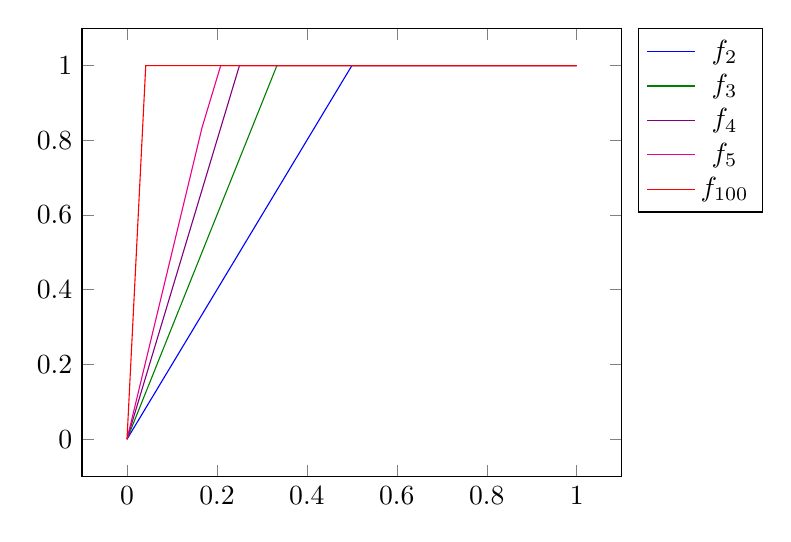
\begin{tikzpicture}
\begin{axis}[domain=0:1, legend pos=outer north east]
\addplot[blue]{2*x*(x<=1/2)+1*(x>1/2)};
\addplot[green!50!black]{3*x*(x<=1/3)+1*(x>1/3)};
\addplot[violet]{4*x*(x<=1/4)+1*(x>1/4)};
\addplot[magenta]{5*x*(x<=1/5)+1*(x>1/5)};
\addplot[red]{100*x*(x<=1/100)+1*(x>1/100)};
\legend{\(f_2\), \(f_3\), \(f_4\), \(f_5\), \(f_{100}\)}
\end{axis}
\end{tikzpicture}
\end{center}
It can be shown that
\[
\lim_{n\to \infty}f_n(x)=f(x)=\begin{cases}
0&\text{if \(x=0\)}, \\
1&\text{if \(x>0\)}.
\end{cases}
\]
\begin{center}
\begin{tikzpicture}
\begin{axis}[domain=0:1, legend pos=outer north east, ymin=-0.1]
\addplot[brown, very thick, domain=0.01:1]{1};
\draw[brown, fill] (0,0) circle [radius=0.8mm];
\draw[brown] (0,1) circle [radius=0.8mm];
\addplot[red]{100*x*(x<=1/100)+1*(x>1/100)};
\draw[-Latex, violet] (0.1,0.1) -- (0.01,0.05);
\draw[-Latex, violet] (0.1,0.1) -- (0.02,0.1);
\draw[-Latex, violet] (0.1,0.1) -- (0.03,0.15);
\node[] () at (0.43,0.1) {still far from \(f(x)=1\)};
\legend{\(f\), \(f_{100}\)}
\end{axis}
\end{tikzpicture}
\end{center}
So, \(\{f_n\}\) converges pointwisely to \(f\) on \(S\). However, the
convergence turns out to be not uniform. For example, take \(N=100\) and
consider \(f_{N}=f_{100}\). For any \(x\in [1/100,1]\), we have
\(f_{100}(x)=f(x)\), so for these \(x\) the pointwise convergence has already
been ``completed''. On the other hand, for any \(0<x<1/100\), \(f_{100}(x)\)
still has a certain distance from the limit \(f(x)=1\), and particularly,
\(f_{100}(x)\) is still very close to \(0\) for very small \(x\). In this
sense, the convergence is not ``uniform''. Note that similar phenomenon occurs
for other \(N\) also.

\item Let us now define the notion of uniform convergence. A sequence of
functions \(\{f_n\}\) on \(S\) \defn{converges uniformly} on \(S\) to a
function \(f\) defined on \(S\), written as ``\(\{f_n\}\to f\text{ uniformly on
\(S\)}\)'', if for any \(\varepsilon>0\), there exists
\(N=N(\varepsilon)\in\N\) such that
\[
|f_{n}(x)-f(x)|<\varepsilon
\]
for any \(n\ge N\) and any \(x\in S\). If \(\{f_n\}\to f\) uniformly on \(S\)
for some function \(f\) on \(S\), we say that \(\{f_n\}\) \defn{converges
pointwisely}/is \defn{uniformly convergent}.


This means that for any point \(x\in S\), \(\{f_n(x)\}\to f(x)\) at a
``uniform'' rate. More specifically, we can always find a sufficiently large
\(N\) that ``works'' for every \(x\in S\), i.e., from the \(N\)th function onward
(\(f_{N}, f_{N+1},\dotsc\)), the value taken at \underline{every} \(x\in S\) is
very close to the corresponding limit \(f(x)\) (within a threshold
\(\varepsilon\)). There is no point \(x\in S\) at which it is still ``far from
convergence''.

It is not hard to see that uniform convergence implies pointwise convergence
(to the same limit), just like how uniform continuity implies continuity.

\item Here we introduce several criteria for uniform convergence.

\begin{proposition}
\label{prp:uniform-conv-crit}
Let \(\{f_n\}\) be a sequence of functions on \(S\). Then the following are
equivalent.
\begin{enumerate}
\item \(\{f_n\}\to f\) uniformly on \(S\).
\item For any \(\varepsilon>0\), there exists \(N\in\N\) such that
\[
\sup\{|f_n(x)-f(x)|:x\in S\}<\varepsilon
\]
for any \(n\ge N\).
\item \(\lim_{n\to \infty}\sup\{|f_n(x)-f(x)|:x\in S\}=0\).
\end{enumerate}
\end{proposition}
\begin{pf}
\underline{\(\text{(b)}\iff\text{(c)}\)}: It follows from the definition of
limit of a sequence of real numbers, since \(\{\sup\{|f_n(x)-f(x)|:x\in
S\}\}_{n=1}^{\infty}\) is just a sequence of real numbers.

\underline{\(\text{(a)}\implies \text{(b)}\)}: Suppose \(\{f_n\}\to f\)
uniformly on \(S\). Then for any \(\varepsilon>0\), there exists \(N\in\N\)
such that
\[
|f_n(x)-f(x)|<\varepsilon/2
\]
for any \(n\ge N\) and any \(x\in S\). Thus, \(\sup\{|f_n(x)-f(x)|:x\in
S\}\le\varepsilon/2<\varepsilon\) for any \(n\ge N\).

\underline{\(\text{(b)}\implies \text{(a)}\)}: For any \(\varepsilon>0\), we
have \(|f_n(x)-f(x)|\le\sup\{|f_n(x)-f(x)|:x\in S\}<\varepsilon\) for any
\(n\ge N\) and any \(x\in S\). The uniform convergence then follows.
\end{pf}

\item Intuitively, if a sequence of functions converges uniformly, the
behaviour of the functions can be ``controlled'' in a uniform manner, and there
would not be abrupt changes in the behaviour in some ``parts'' of the input.
Consequently, some common properties can be ``passed'' to the limiting
function.

The first property that can be ``passed'' is continuity at a point.
\begin{proposition}
\label{prp:unif-conv-seq-cts}
Suppose that \(\{f_n\}\to f\) uniformly on \(S\), and \(f_n\) is continuous at
\(c\in S\) for every \(n\in\N\). Then \(f\) is also continuous at \(c\).
\end{proposition}
\begin{pf}
Fix any \(\varepsilon>0\), from the uniform convergence, there exists
\(N\in\N\) such that \(|f_N(x)-f(x)|<\varepsilon/3\) for any \(x\in S\).

By the continuity of \(f_N\) at \(c\), there exists
\(\delta=\delta(\varepsilon,c)>0\) such that \(|f_N(x)-f_N(c)|<\varepsilon/3\)
for any \(x\in S\) with \(d(x,c)<\delta\).

Thus, for any \(x\in S\) with \(d(x,c)<\delta\), we have
\[
|f(x)-f(c)|\le |f(x)-f_N(x)|+|f_N(x)-f_N(c)|+|f_N(c)-f(c)|
<\frac{\varepsilon}{3}+\frac{\varepsilon}{3}+\frac{\varepsilon}{3}
=\varepsilon.
\]
\end{pf}

\begin{note}
Note that \(\{f_n\}\to f\) uniformly on \(S\) implies that \(\lim_{n\to
\infty}f_n(x)=f(x)\) for any \(x\in S\). Hence, symbolically, we can write
\[
\lim_{n\to \infty}\lim_{x\to c}f_n(x)=\lim_{n\to \infty}f_n(c)
=f(c)=\lim_{x\to c}f(x)=\lim_{x\to c}\lim_{n\to \infty}f_n(x),
\]
which means that ``\(\lim_{n\to \infty}\)'' commutes with ``\(\lim_{x\to c}\)''
under uniform convergence.
\end{note}
\item Next, we show that uniform continuity can be ``passed'' to the limiting
function as well.
\begin{proposition}
\label{prp:unif-conv-seq-unif-cts}
Suppose that \(\{f_n\}\to f\) uniformly on \(S\), and \(f_n\) is uniformly
continuous on \(S\) for every \(n\in\N\). Then \(f\) is also uniformly
continuous on \(S\).
\end{proposition}
\begin{pf}
(Similar to the proof for \Cref{prp:unif-conv-seq-cts}) Fix any
\(\varepsilon>0\). There exists \(N\in\N\) such that
\(|f_N(x)-f(x)|<\varepsilon/3\) for any \(x\in S\).

By the uniform continuity of \(f_N\), there exists \(\delta=\delta(\varepsilon)>0\) such that
\(|f_N(x)-f_N(y)|<\varepsilon/3\) for any \(x,y\in S\) with \(d(x,y)<\delta\).

Hence, for any \(x,y\in S\) with \(d(x,y)<\delta\),
\[
|f(x)-f(y)|\le |f(x)-f_N(x)|+|f_N(x)-f_N(y)|+|f_N(y)-f(y)|
<\frac{\varepsilon}{3}+\frac{\varepsilon}{3}+\frac{\varepsilon}{3}
=\varepsilon.
\]
\end{pf}

\item In \Cref{subsect:conv-ms}, we have introduced the concept of convergence
in a metric space. By considering a metric space of functions equipped with
some metric, we can also talk about convergence for a sequence in functions.
How is the uniform convergence related to the convergence in this metric space
sense? The following theorem suggests the relationship.

\begin{theorem}
\label{thm:unif-conv-ms-conv}
Let \(\{f_n\}\) be a sequence in the metric space \((C_{\mathrm{bd}}(S),d)\)
where \(C_{\mathrm{bd}}(S)\) denotes the set of all bounded continuous
real-valued functions on \(S\) and
\[
d(f,g)=\sup\{|f(x)-g(x)|:x\in S\}
\]
(the \(L^{\infty}\) norm introduced in \labelcref{it:fun-ms-lp-norm}). Then,
\(\{f_n\}\to f\) uniformly on \(X\) iff \(\{d(f_n,f)\}\to 0\), i.e.,
\(\{f_n\}\to f\) in the metric space \((C_{\mathrm{bd}}(S),d)\).
\end{theorem}
\begin{pf}
It follows directly from \Cref{prp:uniform-conv-crit}.
\end{pf}

\begin{remark}
\item In view of this result, the metric \(d\) here is sometimes called the
\defn{uniform metric}.
\item Under the special case where \(S\) is compact, we have
\(C_{\mathrm{bd}}(S)=C(S)\), since all continuous real-valued functions on
\(S\) must be bounded by \Cref{cor:cts-cpt-bounded}.
\end{remark}

\item Recall from \Cref{subsect:complete-ms} that convergence implies
Cauchyness, and the converse holds only when the underlying metric space is
complete. But it turns out that for a sequence of functions on \(S\), uniform
convergence is \emph{equivalent} to ``uniform Cauchyness'', regardless of the
completeness of the underlying metric space.

A sequence of functions \(\{f_n\}\) is \defn{uniformly Cauchy} on \(S\) if for
any \(\varepsilon>0\), there exists \(N=N(\varepsilon)\in\N\) such that
\[
|f_n(x)-f_m(x)|<\varepsilon
\]
for any \(n,m\ge N\) and any \(x\in S\).

The following theorem establishes the equivalence between uniform convergence
and uniform Cauchyness.

\begin{theorem}[Cauchy's criterion for uniform convergence of sequences of functions]
\label{thm:cauchy-crit-seq-unif-conv}
Let \(\{f_n\}\) be a sequence of functions on \(S\). Then, \(\{f_n\}\to f\)
uniformly on \(S\) for some function \(f\) iff \(\{f_n\}\) is uniformly Cauchy
on \(S\).
\end{theorem}
\begin{pf}
``\(\Rightarrow\)'': Assume \(\{f_n\}\to f\) uniformly on \(S\). Fix any
\(\varepsilon>0\), and there exists \(N=N(\varepsilon)\in\N\) such that
\(|f_n(x)-f(x)|<\varepsilon/2\) for any \(n\ge N\) and any \(x\in S\). By
triangle inequality, for any \(m,n\ge N\), we have
\[
|f_n(x)-f_m(x)|\le |f_n(x)-f(x)|+|f_m(x)-f(x)|<\frac{\varepsilon}{2}+\frac{\varepsilon}{2}=\varepsilon.
\]

``\(\Leftarrow\)'': Under the uniform Cauchyness, for any \(x\in S\),
\(\{f_n(x)\}\) is Cauchy in \(\R\), thus converges to \(f(x)\triangleq
\lim_{m\to \infty}f_m(x)\).

Fix any \(\varepsilon>0\). Due to the uniform Cauchyness, there exists
\(N=N(\varepsilon)\in\N\) such that \(|f_n(x)-f_m(x)|<\varepsilon/2\) for any
\(m,n\ge N\) and \(x\in S\). Therefore, for any \(n\ge N\), we have
\[
|f_n(x)-f(x)|=\lim_{m\to \infty}|f_n(x)-f_m(x)|\le\varepsilon/2<\varepsilon,
\]
establishing the uniform convergence.
\end{pf}

\begin{note}
Although we do not require completeness for the metric space \(X\), of which
\(S\) is a subset for this result, it is important that the functions are
real-valued so that the codomain is \(\R\), which is complete.
\end{note}

\item As a corollary, we can show that \((C_{\mathrm{bd}}(S),d)\), where \(d\)
is the uniform metric, is a complete metric space.

\begin{corollary}
\label{cor:cbd-ms-unif-complete}
Let \((C_{\mathrm{bd}}(S),d)\) be the metric space as defined in
\Cref{thm:unif-conv-ms-conv}. Then \((C_{\mathrm{bd}}(S),d)\) is complete.
\end{corollary}
\begin{pf}
Fix any Cauchy sequence \(\{f_n\}\) in \(C_{\mathrm{bd}}(S)\). Then for any
\(\varepsilon>0\), there exists \(N\in\N\) such that
\[
|f_n(x)-f_m(x)|\le d(f_n,f_m)<\varepsilon
\]
for any \(m,n\ge N\) and \(x\in S\). This shows \(\{f_n\}\) is uniformly Cauchy
on \(S\), thus by \Cref{thm:cauchy-crit-seq-unif-conv}, \(\{f_n\}\to f\)
uniformly for some function \(f\). By \Cref{prp:unif-conv-seq-cts}, \(f\) is a
continuous function on \(S\). Next, due to the uniform convergence, there
exists \(N\in\N\) such that \(|f_N(x)-f(x)|<1\) for any \(x\in S\). Since
\(f_N\) is bounded, \(|f_N(x)|\le M\) for some \(M>0\). Hence by triangle
inequality, \(|f(x)|= |f_N(x)|+|f(x)-f_N(x)|< M+1\) for any \(x\in S\), meaning
that \(f\) is bounded.  Thus, \(f\in C_{\mathrm{bd}}(S)\).

By \Cref{thm:unif-conv-ms-conv}, we know that \(\{d(f_n,f)\}\to 0\), thus
\(\{f_n\}\to f\in C_{\mathrm{bd}}(S)\) by \labelcref{it:ms-conv-relate-real-conv}. This
shows \(\{f_n\}\) is convergent in \(C_{\mathrm{bd}}(S)\).
\end{pf}

\item Before going further into the discussion about uniform convergence, we
shall apply the concepts we learn here to prove a result concerning the
existence and uniqueness of solutions to ODEs, which illustrates a
``practical'' application of the abstract concepts here.

\begin{theorem}[Picard-Lindel\"of theorem]
\label{thm:picard-lindelof}
Let \(I\) and \(J\) be open intervals in \(\R\) containing a constant
\(m_0\in\R\) and \(0\) respectively.  Let \(F:I\times J\to\R\) be a
continuously differentiable\footnote{It means that (i) \(F\) is differentiable
and (ii) the two partial derivatives of \(F\) are continuous.} function. Then
there exists \(\delta>0\) such that, over \((-\delta,\delta)\), there is a
unique function \(f\) such that \(f(0)=m_0\) and
\(f'(t)=F(f(t),t)\).\footnote{This means \(f\) ``locally solves'' the initial value
problem specified here near \(0\), uniquely.}
\begin{center}
\begin{tikzpicture}
\draw[green!50!black, dashed] (-2,-2) rectangle (4,2);
\node[green!50!black] () at (1,2.5) {\(I\times J\)};
\draw[brown, fill] (1,0) circle [radius=0.8mm];
\node[brown] () at (1.7,-0.5) {\((m_0,0)\)};
\draw[blue] (0.8,-0.5) .. controls (1.2,0.3) and (0.9,0.4) .. (1.3,0.5);
\node[blue] () at (1.5,0.7) {\small{\((f(t),t)\)}};
\draw[-Latex, violet] (1.1,0.4) to[bend left] node[auto, swap]{\(F\)} (5,1.5);
\node[violet] () at (5.5,1.5) {\(f'(t)\)};
\end{tikzpicture}
\end{center}
\end{theorem}
\begin{pf}
First note that
\begin{align*}
&\qquad f(0)=m_0\qqtext{and}f'(s)=F(f(s),s) \\
&\iff f(t)=m_0+\int_{0}^{t}F(f(s),s)\dd{s} \\
&\iff f \text{ is a fixed point of }\Lambda\text{ where
}\Lambda(\vc{g})=m_0+\int_{0}^{t}F(\vc{g}(s),s)\dd{s}.
\end{align*}
We then reduced the problem to finding a unique fixed point, for which the
\emph{Banach's fixed point theorem} would be helpful.

Up to passing \(I\) and \(J\) to subintervals such that \(I\times J\) still
contains \((m_0,0)\), we can assume that \(M=\sup_{(x,y)\in I\times
J}|F(x,y)|<\infty\) and \(M'=\sup_{(x,y)\in I\times J}|\partial_1 F|<\infty\)
(where \(\partial_1 F\) denotes the partial derivative of \(F\) with respect to
its first argument). Choose \(
\delta=\min\qty{\frac{1}{M},\frac{1}{2M'}}\) (for reasons that will become
transparent very soon).

Consider the metric space \(C([-\delta,\delta])\) (the set of all real-valued
continuous functions on \([-\delta,\delta]\)) with the uniform metric \(d\),
and consider the closed ball \(\overline{B}(m_0,1)\subseteq
C([-\delta,\delta])\) where ``\(m_0\)'' here denotes the constant function on
\([-\delta,\delta]\) that always takes the value of \(m_0\). We define
\(\Lambda\) on the closed ball \(\overline{B}(m_0,1)\).

For any \(g\in\overline{B}(m_0,1)\subseteq C([-\delta,\delta])\) and any
\(t\in[-\delta,\delta]\),
\[
|\Lambda(g)(t)-m_0|
=\qty|\int_{0}^{t}F(g(s),s)\dd{s}|
\le |t|M
\le \delta M
\le 1.
\]
This shows \(\Lambda(g)\in\overline{B}(m_0,1)\), so we can define \(\Lambda\)
as a function from \(\overline{B}(m_0,1)\) to \(\overline{B}(m_0,1)\).

Next, we want to show that \(\Lambda\) is a contraction of
\(\overline{B}(m_0,1)\). Consider
\begin{align*}
d(\Lambda(g),\Lambda(h))
&=\sup_{t\in[-\delta,\delta]}|\Lambda(g)(t)-\Lambda(h)(t)| \\
&=\sup_{t\in[-\delta,\delta]}\qty|\int_{0}^{t}[F(g(s),s)-F(h(s),s)]\dd{s}| \\
&\le\sup_{t\in[-\delta,\delta]}\int_{0}^{t}|F(g(s),s)-F(h(s),s)|\dd{s}.
\end{align*}
For the integrand, applying mean value theorem on the first argument of \(F\)
(with the second argument fixed), there exists \(v\in (g(s),h(s))\) such that
\(\partial_1 F(v,s)(g(s)-h(s))\le M'[g(s)-h(s)]\).

Thus, we can write
\begin{align*}
\sup_{t\in[-\delta,\delta]}\int_{0}^{t}|F(g(s),s)-F(h(s),s)|\dd{s}
&\le\sup_{t\in[-\delta,\delta]}\int_{0}^{t}M'\underbrace{|g(s)-h(s)|}_{d(g,h)}\dd{s} \\
&\le \sup_{t\in[-\delta,\delta]}\underbrace{M'\delta d(g,h)}_{\text{free of \(t\)}} \\
&=M'\delta d(g,h) \\
&\le \frac{1}{2}d(g,h),
\end{align*}
so \(\Lambda\) is a contraction of \(\overline{B}(m_0,1)\).

As \([-\delta,\delta]\) is compact in \(\R\), every continuous real-valued
function on \([-\delta,\delta]\) is bounded, by \Cref{cor:cts-cpt-bounded}.
Thus \(C([-\delta,\delta])=C_{\mathrm{bd}}([-\delta,\delta])\). Then by
\Cref{cor:cbd-ms-unif-complete}, \((C([-\delta,\delta]),d)\) is
complete. Since \(\overline{B}(m_0,1)\) is a closed subset of
\(C([-\delta,\delta])\), it follows by \Cref{prp:cls-subset-cpl-ms-cpl} that
the metric subspace \((\overline{B}(m_0,1),d)\) (with the induced uniform
metric \(d\)) is complete also.

It then follows by Banach's fixed point theorem (\Cref{thm:banach-fixed-pt})
that \(\Lambda\) has a unique fixed point, namely the function \(f\).
\end{pf}

\end{enumerate}

\subsection{Uniform Convergence of Series of Functions}
\begin{enumerate}
\item Now we go back to the discussion about uniform convergence. After
considering \emph{sequences} of functions, we consider \emph{series} of
functions. A familiar example of series of functions is the exponential
function:
\[
e^{x}=\sum_{k=0}^{\infty}\frac{x^k}{k!}=\sum_{k=0}^{\infty}f_k(x),
\]
where \(f_k(x)=x^k/k!\) for any \(k\in\N_0\). Each term in the infinite sum can
be regarded as a function in \(x\). How to ``make sense of'' this kind of
infinite sum?

\item Like how we handle series of real numbers in MATH2241, we start with
\emph{partial sums}. For every \(k\in\N\), let \(f_k:S\to\R\) be a function.
For any \(n\in\N\), define the \defn{\(n\)th partial sum} of the series
\(\sum_{k=1}^{\infty}f_k\) as the function \(s_n:S\to\R\) given by
\[
s_n(x)=\sum_{k=1}^{n}f_k(x)\quad\text{for any \(x\in S\)}.
\]

\item After that, we can define \emph{uniform convergence} for series,
utilizing the concept of uniform convergence of sequences of functions. The
infinite series \(\sum_{k=1}^{\infty}f_k\) \defn{converges uniformly} on \(S\)
if there exists a function \(f:S\to\R\) such that \(\{s_n\}\to f\) uniformly on
\(S\).  In this case, we write ``\(\sum_{k=1}^{\infty}f_k(x)=f(x)\) uniformly
on \(S\)''.

Analogously, if there is a function \(f:S\to\R\) such that \(\{s_n\}\to f\)
\emph{pointwisely} on \(S\), then we say that the infinite series
\(\sum_{k=1}^{\infty}f_k\) \defn{converges pointwisely} on \(S\), written as
``\(\sum_{k=1}^{\infty}f_k(x)=f(x)\) pointwisely on \(S\)''.

Again, if \(\sum_{k=1}^{\infty}f_k(x)=f(x)\) uniformly (pointwisely resp.) on
\(S\) for some function \(f:S\to\R\), we say that \(\{f_n\}\) \defn{converges
uniformly} (\defn{converges pointwisely} resp.)/is \defn{uniformly convergent}
(\defn{pointwisely convergent} resp.).

It turns out that in the case of exponential function, the series
\(\sum_{k=0}^{\infty}\frac{x^k}{k!}\)\footnote{We may change the index to make
the sum starts at \(k=1\) to match with the discussion above.} converges
uniformly on any finite interval in \(\R\). The limiting function in the
uniform convergence sense can then be \emph{defined} as the exponential
function. This gives rise to one approach of defining exponential function.

\item For uniform convergence of infinite series of functions, we also have a
Cauchy's criterion.

\begin{theorem}[Cauchy's criterion for uniform convergence of series of functions]
\label{thm:cauchy-crit-series-uniform-conv}
The infinite series \(\sum_{k=1}^{\infty}f_k\) converges uniformly on \(S\) iff
for any \(\varepsilon>0\), there exists \(N\in\N\) such that
\[
\qty|\sum_{k=n+1}^{m}f_k(x)|<\varepsilon
\]
for any \(m>n\ge N\) and \(x\in S\).
\end{theorem}
\begin{pf}
Consider
\begin{align*}
&\qquad\text{\(\sum_{k=1}^{\infty}f_k\) converges uniformly on \(S\)}\\
&\iff \text{\(\{s_n\}\to f\) uniformly on \(S\) for some function \(f:S\to\R\)} \\
&\iff \text{\(\{s_n\}\) is uniformly Cauchy on \(S\)} \qquad\text{(\Cref{thm:cauchy-crit-seq-unif-conv})} \\
&\iff \text{for any \(\varepsilon>0\), there exists \(N\in\N\) such that
\(|s_m(x)-s_n(x)|<\varepsilon\) for any \(m>n\ge N\) and \(x\in S\)} \\
&\iff \text{for any \(\varepsilon>0\), there exists \(N\in\N\) such that
\(\qty|\sum_{k=n+1}^{m}f_k(x)|<\varepsilon\) for any \(m>n\ge N\) and \(x\in
S\)}.
\end{align*}
\end{pf}

\item It turns out that like uniform convergence of sequences of functions, the
property of continuity at a point can be ``passed'' to the limiting function,
under the uniform convergence of series of functions.

\begin{proposition}
\label{prp:unif-conv-series-cts}
Suppose that \(f_k\) is continuous at \(c\in S\) for every \(k\in\N\), and
\(\sum_{k=1}^{\infty}f_k(x)=f(x)\) uniformly on \(S\). Then \(f\) is also
continuous at \(c\).
\end{proposition}
\begin{pf}
By assumption, the sequence of partial sums \(\{s_n\}\to f\) uniformly on
\(S\). Since \(f_k\) is continuous at \(c\in S\) for each \(k\in\N\), the same
is true for every partial sum \(s_n\).

Thus, applying \Cref{prp:unif-conv-seq-cts} on \(\{s_n\}\) suggests that \(f\)
is continuous at \(c\).
\end{pf}

\item Apart from the Cauchy's criterion
(\Cref{thm:cauchy-crit-series-uniform-conv}), the following result is also an
useful test of uniform convergence of series of functions.

\begin{theorem}[Weierstrass M-test]
\label{thm:weierstrass-m-test}
Let \(\sum_{k=1}^{\infty}f_k\) be a series of functions satisfying
\begin{enumerate}
\item \(|f_k(x)|\le M_k\) for any \(k\in\N\) and \(x\in X\), and
\item \(\sum_{k=1}^{\infty}M_k\) converges.
\end{enumerate}
Then, \(\sum_{k=1}^{\infty}f_k\) converges uniformly on \(X\).
\end{theorem}
\begin{pf}
Fix any \(\varepsilon>0\).  Since \(\sum_{k=1}^{\infty}M_k\) converges, there
exists \(N\in\N\) such that
\(\qty|\sum_{k=1}^{\infty}M_k-\sum_{k=1}^{N}M_k|=\sum_{k=N+1}^{\infty}M_k<\varepsilon\).\footnote{Note
that \(M_k\ge 0\) for any \(k\in\N\) due to (a).} Thus, for any \(m>n\ge N\)
and \(x\in S\),
\[
\qty|\sum_{k=n+1}^{m}f_k(x)|
\le\sum_{k=n+1}^{m}|f_k(x)|
\le \sum_{k=n+1}^{m}M_k
\le \sum_{k=N+1}^{\infty}M_k
<\varepsilon,
\]
and then the uniform convergence follows from
\Cref{thm:cauchy-crit-series-uniform-conv}.
\end{pf}
\end{enumerate}

\subsection{Commutativity of Limit with Integration/Differentiation}
\begin{enumerate}
\item Next, we are going to investigate questions concerning the validity of
``switching orders of limit and integration/differentiation'':
\begin{enumerate}[label={Q\arabic*}]
\item \label{it:switch-int-lim} Is it true that \(\lim_{n\to
\infty}\int_{a}^{b}f_n(x)\dd{x}=\int_{a}^{b}\lim_{n\to \infty}f_n(x)\dd{x}\)?
\item \label{it:switch-diff-lim} Is it true that \(\lim_{n\to
\infty}f_n'(x)=(\lim_{n\to \infty}f_n(x))'\)?
\end{enumerate}
\begin{note}
Here ``\(\lim_{n\to \infty}\)'' is the usual limit for real numbers, and note
that the function \(f\) defined by \(f(x)=\lim_{n\to \infty}f_n(x)\) is the
\emph{pointwise} limit of \(\{f_n\}\).
\end{note}

\item Unfortunately, in general the answers to both
\labelcref{it:switch-int-lim,it:switch-diff-lim} are negative, as the following
examples illustrate.
\begin{itemize}
\item \emph{Negative example for Q1:} For any \(n\in\N\), define
\(f_n:[0,1]\to\R\) by \(f_n(x)=n^{2}(1-x)x^{n}\) for any \(x\in[0,1]\). Then,
note that \(\{f_n\}\to f\equiv 0\) pointwisely on \([0,1]\).

Now for any \(n\in\N\), compute
\[
\int_{0}^{1}f_n(x)\dd{x}=\frac{n^{2}}{(n+1)(n+2)},
\]
and thus
\[
\lim_{n\to \infty}\int_{0}^{1}f_n(x)\dd{x}
=\lim_{n\to\infty}\frac{n^{2}}{(n+1)(n+2)}
=\lim_{n\to\infty}\frac{1}{1+3/n+2/n^2}
=1\ne 0=\int_{0}^{1}f(x)\dd{x}.
\]
\item \emph{Negative example for Q2:} For any \(n\in\N\), define
\(f_n:\R\to\R\) by \(f_n(x)=\frac{1}{\sqrt{n}}\sin nx\) for any
\(x\in \R\). Note that for any \(x\in\R\), we have
\[
|f_n(x)|=\qty|\frac{1}{\sqrt{n}}\sin nx|\le\qty|\frac{1}{\sqrt{n}}|.
\]
Hence, by sandwich theorem, \(\lim_{n\to \infty}f_n(x)=0\), and thus
\(\{f_n\}\to f\equiv 0\) pointwisely on \(\R\).

Clearly we have \(f'(x)=0\) for any \(x\in\R\). But for any \(x\in\R\), we have
\(f_n'(x)=\sqrt{n}\cos nx\), and hence \(\lim_{n\to \infty}f_n'(x)\) does not
exist.
\end{itemize}

\item Nevertheless, the answers can become affirmative with some additional
conditions imposed. For \labelcref{it:switch-int-lim}, the answer is
affirmative under uniform convergence.

\begin{proposition}
\label{prp:unif-conv-lim-int-comm}
Let \(\{f_n\}\) be a sequence of continuous functions on \([a,b]\) which
converges uniformly to \(f\) on \([a,b]\). Then,
\[
\lim_{n\to \infty}\int_{a}^{b}f_n(x)\dd{x}
=\int_{a}^{b}f(x)\dd{x}
=\int_{a}^{b}\lim_{n\to \infty}f_n(x)\dd{x}.
\]
\end{proposition}
\begin{pf}
The second equality follows from the uniform convergence, so it suffices to
prove the first.

Firstly, by \Cref{prp:unif-conv-seq-cts}, the uniform limit \(f\) is continuous. Since continuity implies (Riemann) integrability, all \(f_n\)'s and \(f\) are integrable over \([a,b]\).

Now, using the assumption that \(\{f_n\}\to f\) uniformly on \([a,b]\), we have for any \(\varepsilon>0\), there exists \(N\in\N\) such that
\[
|f_n(x)-f(x)|<\frac{\varepsilon}{2(b-a)}
\]
for any \(n\ge N\) and \(x\in [a,b]\). It then follows that
\[
\qty|\int_{a}^{b}f_n(x)\dd{x}-\int_{a}^{b}f(x)\dd{x}|
=\qty|\int_{a}^{b}f_n(x)-f(x)\dd{x}|
\le\int_{a}^{b}|f_n(x)-f(x)|\dd{x}
\le\frac{\varepsilon}{2}
<\varepsilon.
\]
\end{pf}
\item Although the uniform convergence ensures the commutativity of limit with
integration, this condition is not a necessary condition. 

Example: For any \(n\in\N\), define \(f_n:[0,1]\to\R\) by \(f_n(x)=x^n\) for
any \(x\in [0,1]\). Then, \(\{f_n\}\to f\) pointwisely on \([0,1]\) where
\[f(x)=\begin{cases}
0&\text{if \(x\in [0,1)\)}, \\
1&\text{if \(x=1\)}.
\end{cases}
\]
Then, we have
\[
\lim_{n\to \infty}\int_{0}^{1}f_n(x)\dd{x}
=\lim_{n\to \infty}\frac{1}{n+1}
=0=\int_{0}^{1}f(x)\dd{x}.
\]
Although the limit is commutative with integration here, the convergence
\(\{f_n\}\to f\) is not uniform.

\item Now, we consider \labelcref{it:switch-diff-lim}. Again the answer becomes
affirmative with some additional conditions.

\begin{proposition}
\label{prp:unif-conv-lim-diff-comm}
Let \(\{f_n\}\) be a sequence of differentiable functions on a bounded open
interval \(S=(a,b)\) where \(a<b\). Suppose that
\begin{enumerate}[label={(\roman*)}]
\item \(\{f_n'\}\to g\) uniformly on \(S\) for some function \(g\), and
\item there exists \(x_0\in S\) such that \(\{f_n(x_0)\}\) converges.
\end{enumerate}
Then,
\begin{enumerate}
\item \(\{f_n\}\to f\) uniformly on \(S\) for some function \(f\), and
\item \(f\) is differentiable, with \((\lim_{n\to \infty}f_n(x))'=f'(x)=g(x)=\lim_{n\to \infty}f_n'(x)\) for any \(x\in S\).
\end{enumerate}
\end{proposition}
\begin{pf}
Fix any \(c\in (a,b)\). For any \(n\in\N\), we define \(g_n:S\to\R\) by
\[
g_n(x)=\begin{cases}
\frac{f_n(x)-f_n(c)}{x-c}&\text{if \(x\ne c\)}, \\
f_n'(c)&\text{if \(x=c\)}.
\end{cases}
\]
By construction, \(g_n\) is continuous at \(c\).

By mean value theorem, for any \(x\ne c\),
\begin{align*}
|g_n(x)-g_m(x)|&=\qty|\frac{[f_n(x)-f_m(x)]-[f_n(c)-f_m(c)]}{x-c}| \\
&=\qty|\frac{(f_n-f_m)(x)-(f_n-f_m)(c)}{x-c}| \\
&=|(f_n-f_m)'(t)| \\
&=|f_n'(t)-f_m'(t)|
\end{align*}
for some \(t\) between \(x\) and \(c\).

Since \(\{f_n'\}\) converges uniformly on \(S\), it is uniformly Cauchy on
\(S\). Thus, for any \(\varepsilon>0\), there exists \(N\in\N\) such that for any \(m,n\ge N\),
\[
|f_n'(x)-f_m'(x)|<\varepsilon
\]
for any \(x\in S\). It then follows that for any \(m,n\ge N\),
\[
|g_n(x)-g_m(x)|=\begin{cases}
|f_n'(t)-f_m'(t)|&\text{if \(x\ne c\)}, \\
|f_n'(c)-f_m'(c)|&\text{if \(x=c\)}
\end{cases}
<\varepsilon
\]
for any \(x\in S\), hence \(\{g_n\}\) is uniformly Cauchy.
\begin{enumerate}
\item We take \(c=x_0\) for each \(g_n\) defined above. For any \(m,n\in\N\), we
have
\begin{align*}
f_n(x)-f_m(x)&=[f_n(x_0)+g_n(x_0)(x-x_0)]-[f_m(x_0)+g_m(x_0)(x-x_0)] \\
&=f_n(x_0)-f_m(x_0)+(x-x_0)(g_n(x)-g_m(x))
\end{align*}
for any \(x\in S\). Since \(\{f_n(x_0)\}\) converges, there exists \(N_1\in\N\)
such that
\[
|f_n(x_0)-f_m(x_0)|<\varepsilon/2
\]
for any \(n,m\ge N_1\). On the other hand, since \(\{g_n\}\) is uniformly
Cauchy on \(S\), there exists \(N_2\in\N\) such that
\[
|g_n(x)-g_m(x)|<\frac{\varepsilon}{2(b-a)}
\]
for any \(m,n\ge N_2\) and any \(x\in S\).

It follows that for any \(m,n\ge \max\{N_1,N_2\}\),
\begin{align*}
|f_n(x)-f_m(x)|&\le |f_n(x_0)-f_m(x_0)|+|x-x_0||g_n(x)-g_m(x)| \\
&<\frac{\varepsilon}{2}+(b-a)\cdot \frac{\varepsilon}{2(b-a)} \\
=\varepsilon,
\end{align*}
for any \(x\in S\). Thus, \(\{f_n\}\) is uniformly Cauchy, hence converges
uniformly to some function \(f\) by \Cref{thm:cauchy-crit-seq-unif-conv}.
\item For any \(c\in S\), we have
\begin{align*}
f'(c)&=\lim_{x\to c}\frac{f(x)-f(c)}{x-c} \\
&=\lim_{x\to c}\lim_{n\to \infty}\frac{f_n(x)-f_n(c)}{x-c} \\
&=\lim_{n\to \infty}\lim_{x\to c}\frac{f_n(x)-f_n(c)}{x-c} &\text{(by \Cref{prp:unif-conv-seq-cts})}\\
&=\lim_{n\to \infty}\lim_{x\to c}g_n(x) \\
&=\lim_{n\to \infty}g_n(c)&\text{(\(g_n\) is continuous)} \\
&=\lim_{n\to \infty}f'(c) \\
&=g(c).
\end{align*}
\end{enumerate}
\end{pf}
\item Note that in \Cref{prp:unif-conv-lim-diff-comm}, apart from requiring the
uniform convergence of \(\{f_n'\}\), we also need an additional condition that
\(\{f_n(x_0)\}\) converges for some \(x_0\in S\). To illustrate the necessity
of this additional condition, consider the following example.

Let \(S=(0,1)\) and for any \(n\in\N\), define \(f_n(x)=\ln nx\) for any \(x\in
S\).  Note that for each \(n\in\N\), \(f_n\) is differentiable and
\(f_n'(x)=1/x\) for any \(x\in S\). Thus, we have \(\{f_n'\}\to g\) uniformly
on \(S\), where \(g(x)=1/x\) for any \(x\in S\).

However, for any \(x\in S\), \(\{f_n(x)\}\) diverges, so the condition (ii)
fails. So  \Cref{prp:unif-conv-lim-diff-comm} does not apply. Also observe that
since \(\{f_n\}\) does not even converge pointwisely, it does not
converge uniformly.

\item We also have a series version of \Cref{prp:unif-conv-lim-diff-comm}:

\begin{corollary}
\label{cor:series-unif-conv-lim-diff-comm}
Let \(\{f_n\}\) be a sequence of differentiable functions on a bounded open
interval \(S\subseteq \R\). Suppose that
\begin{enumerate}[label={(\roman*)}]
\item \(\sum_{n=1}^{\infty}f_n'(x)=g(x)\) uniformly on \(S\), and
\item there exists \(x_0\in S\) such that \(\sum_{n=1}^{\infty}f_n(x_0)\)
converges.
\end{enumerate}
Then,
\begin{enumerate}
\item \(\sum_{n=1}^{\infty}f_n(x)=f(x)\) uniformly on \(S\), and
\item \(f\) is differentiable, with \(f'(x)=\sum_{n=1}^{\infty}f_n'(x)\) for any \(x\in S\).
\end{enumerate}
\end{corollary}
\begin{pf}
For any \(n\in\N\), define the partial sums \(F_n:S\to\R\) by
\(F_n(x)=\sum_{k=1}^{n}f_k(x)\) for any \(x\in S\). Since each \(f_k\) is
differentiable, each \(F_n\) is differentiable.

Also, we have
\[
\{F_n'\}=\qty{\qty(\sum_{k=1}^{n}f_k)'}
=\qty{\sum_{k=1}^{n}f_k'}
\overset{\text{(i)}}{\to}g
\]
uniformly on \(S\). Furthermore, we have
\[
\{F_n(x_0)\}=\qty{\sum_{k=1}^{n}f_k(x_0)}
\overset{\text{(ii)}}{\to}\sum_{k=1}^{\infty}f_k(x_0)\in\R.
\]

So, the conditions (i) and (ii) in \Cref{prp:unif-conv-lim-diff-comm} are
satisfied, and hence there exists a differentiable function \(f:S\to\R\) such that
\[
\sum_{n=1}^{\infty}f_n=\lim_{n\to \infty}F_n=f
\]
uniformly on \(S\), with
\[
f'(x)=g(x)=\sum_{n=1}^{\infty}f_n'(x)
\]
for any \(x\in S\).
\end{pf}
\end{enumerate}
\subsection{Arzel\`a-Ascoli Theorem}
\begin{enumerate}
\item To close \Cref{sect:unif-cont-conv}, we will prove an important theorem
in analysis known as \emph{Arzel\`a-Ascoli theorem}. To motivate the
discussion, we consider its application to partial differential equations
(PDEs). By Picard-Lindel\"of theorem (\Cref{thm:picard-lindelof}), we can
analyze the existence and uniqueness of solutions to ODEs.  But the situation
is much more complicated for PDEs.

To assess the qualitative features of PDEs like existence and uniqueness of
solutions, a possible approach is to first try to find some ``approximated''
solution \(f_n\) for each \(n\in\N\).

Next, we investigate the converging behaviour of \(\{f_n\}\). Sometimes we can
find a convergent subsequence of \(\{f_n\}\) converging to some function \(f\).
If we are ``lucky'' enough, the function \(f\) could be the exact solution to the
PDE. Hence, we are interested in knowing whether a given sequence of functions
\(\{f_n\}\) has a convergent subsequence, and Arzel\`a-Ascoli theorem suggests
a necessary and sufficient condition for it to happen, under some assumptions.

\item Before stating Arzel\`a-Ascoli theorem, we introduce/recall some
terminologies and results related to different kinds of \emph{compactness}. Let
\(X\) be a metric space. A set \(S\subseteq X\)
\begin{enumerate}
\item (recall) is \emph{compact} if every open cover of \(S\) has a finite subcover;
\item (recall) has the \emph{Boltzano-Weierstrass property} or is \emph{limit
point compact} if every infinite subset of \(S\) has an accumulation point in \(S\);
\item is \defn{sequential compact} if every sequence in \(S\) has a subsequence
which is convergent in \(S\);
\item is \defn{relatively sequential compact} if every sequence in \(S\) has a
subsequence which is convergent in \(X\);
\item is \defn{relatively compact} if \(\overline{S}\) is compact.
\end{enumerate}
\begin{theorem}
\label{thm:diff-cpt-relate}
We have \(\text{(a)}\iff\text{(b)}\iff\text{(c)}\implies
\text{(d)}\iff\text{(e)}\).
\end{theorem}
\item Next, we introduce some more terminologies and results for preparation of
the proof of Arzel\`a-Ascoli theorem. Let \(X\) be a metric space.
\begin{itemize}
\item A set \(S\subseteq X\) is \defn{dense} if \(\overline{S}=X\).
\item A set \(\mathcal{F}\subseteq C(X)\) is \defn{pointwise bounded} if for any \(x\in
X\), \(\sup\{|f(x)|:f\in \mathcal{F}\}<\infty\). \begin{note}
\(C(X)\) denotes the set of all continuous real-valued functions on \(X\).
\end{note}
\item A set \(\mathcal{F}\subseteq C(X)\) is \defn{equicontinuous at \(x_0\in
X\)} if for any \(\varepsilon>0\), there exists
\(\delta=\delta(\varepsilon,x_0)>0\) such that for any \(x\in B(x_0,\delta)\),
\(|f(x)-f(x_0)|<\varepsilon\) for any \(f\in \mathcal{F}\).
\begin{intuition}
When \(\mathcal{F}\) is equicontinuous at \(x_0\), all functions in the family
\(\mathcal{F}\) vary over a given neighbourhood of \(x_0\) at an ``equal''
rate.
\end{intuition}

The set \(\mathcal{F}\) is \defn{equicontinuous (on \(X\))} if \(\mathcal{F}\) is
equicontinuous at every point in \(X\).
\end{itemize}

\item Example of being \emph{not} equicontinuous: Let \(S=[0,1]\subseteq \R\)
and define \(f_n:S\to\R\) by
\[
f_n(x)=\begin{cases}
nx&\text{if \(x\in[0,1/n]\)}, \\
1&\text{if \(x\in[1/n,1]\)},
\end{cases}
\]
for any \(n\in\N\).
\begin{center}
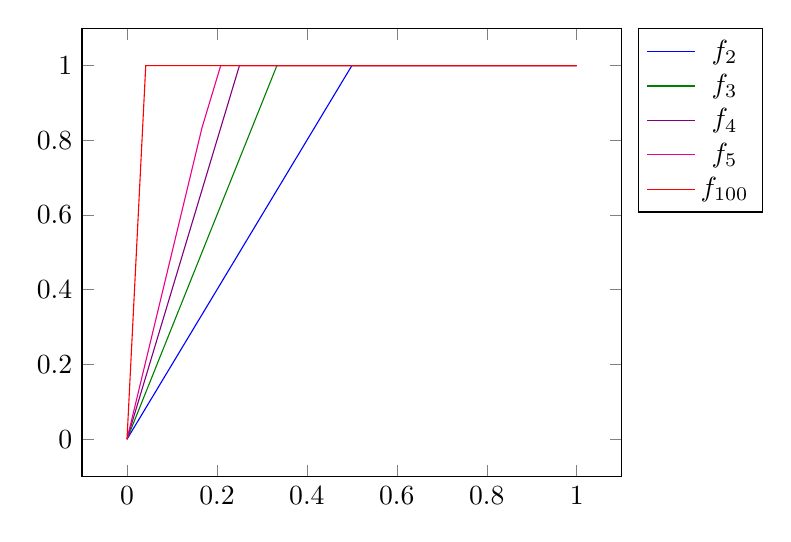
\begin{tikzpicture}
\begin{axis}[domain=0:1, legend pos=outer north east]
\addplot[blue]{2*x*(x<=1/2)+1*(x>1/2)};
\addplot[green!50!black]{3*x*(x<=1/3)+1*(x>1/3)};
\addplot[violet]{4*x*(x<=1/4)+1*(x>1/4)};
\addplot[magenta]{5*x*(x<=1/5)+1*(x>1/5)};
\addplot[red]{100*x*(x<=1/100)+1*(x>1/100)};
\legend{\(f_2\), \(f_3\), \(f_4\), \(f_5\), \(f_{100}\)}
\end{axis}
\end{tikzpicture}
\end{center}

Then, \(\{f_n\}\) is \emph{not} equicontinuous at 0.
\begin{intuition}
The function \(f_n\) changes at a ``faster'' rate around \(0\) as \(n\) gets
large, so the ``rate of change around \(0\)'' is not equal for all functions in
\(\{f_n\}\).
\end{intuition}

\begin{pf}
For any \(\delta>0\), there exists \(N>2/\delta\), which means
\(\delta/2>1/N\). Now consider \(x_N=\min\{\delta/2,1\}\in B(x_0,\delta)\). We
have \(f_N(x_N)=1\) by construction. Next, take \(\varepsilon=1/2\), and then
\(|f_N(x_N)-f_N(0)|=1>\varepsilon\).
\end{pf}

\item A metric space \(X\) is \defn{separable} if it contains a countable dense
subset. Example: \(X=[0,1]\) is separable since \(S=\Q\cap[0,1]\subseteq X\) is
countable and dense.
\begin{lemma}
\label{lma:cpt-separable}
Any compact metric space \(X\) is separable.
\end{lemma}
\begin{pf}
Since \(X\) is compact, for each \(n\in\N\), the open cover \(\{B(x,1/n):x\in
X\}\) of \(X\) has a finite subcover \(\{B(x_i^{(n)},1/n)\}_{i=1}^{m_n}\). Let
\(S_n=\{x_i^{(n)}\}_{i=1}^{m_n}\) denote the set containing all ``centres'' in
the finite subcover.

Then, the union \(S=\bigcup_{n=1}^{\infty}S_n\) is countable and dense.

\underline{Countable}: Since each \(S_n\) is finite, one can use a similar
argument as the proof of countability of \(\Q\).

\underline{Dense}: Fix any \(x\in X\). \vc{For any \(r>0\)}, there exists \(N\in\N\) such
that \(1/N<r\). Since \(\{B(x_i^{(N)},1/N)\}_{i=1}^{m_N}\) covers \(X\), there
exists \(j\in\{1,\dotsc,m_N\}\) such that \(x\in B(x_j^{(N)},1/N)\), which in
turn means that \(x_j^{(N)}\in B(x,1/N)\subseteq B(x,r)\). Thus, \vc{\(B(x,r)\cap
S\ne\varnothing\)}, and so \(x\in\overline{S}\). This shows \(X\subseteq
\overline{S}\), and the reverse subset inclusion is clear since every adherent
point of \(S\) must belong to \(X\) by definition.
\end{pf}

\item Now we will prove Arzel\`a-Ascoli theorem.

\begin{theorem}[Arzel\`a-Ascoli theorem]
\label{thm:arzela-ascoli}
Let \(X\) be a compact metric space, and denote by \(C(X)\) the set of all
real-valued continuous functions on \(X\). Equip \(C(X)\) with the uniform
metric \(d\). Then, the family \(\mathcal{F}\subseteq C(X)\) is relatively
compact iff it is equicontinuous and pointwise bounded.
\end{theorem}
\begin{pf}
``\(\Rightarrow\)'':

\underline{\(\mathcal{F}\) is relatively compact \(\implies\) \(\mathcal{F}\)
is pointwise bounded}:

We prove by contrapositive. Suppose \(\mathcal{F}\) is not pointwise bounded.
Then for some \(x_0\in X\), \(\sup_{f\in\mathcal{F}}|f(x_0)|=\infty\), which
means that there exists \(f_n\in\mathcal{F}\) such that \(|f_n(x_0)|>n\) for
any \(n\in\N\).

This implies that \(\{f_n(x_0)\}\) has no convergent subsequence in \(\R\), and
thus the sequence \(\{f_n\}\) in \(\mathcal{F} \) has no subsequence which is
convergent in \(C(X)\). Hence, \(\mathcal{F}\) is not relatively compact by
\Cref{thm:diff-cpt-relate}.

\underline{\(\mathcal{F}\) is relatively compact \(\implies\) \(\mathcal{F}\)
is equicontinuous}:

We again prove by contrapositive. Suppose \(\mathcal{F}\) is not equicontinuous
at some \(x_0\in X\). Then there exists \(\varepsilon_0>0\) such that for any
\(n\in\N\), there exists \(f_n\in\mathcal{F}\) such that
\(|f_n(x_n)-f_n(x_0)|\mgc{>\varepsilon_0}\) for some \(\mgc{x_n\in B(x_0,1/n)}\).

Now assume to the contrary that \(\mathcal{F}\) is relatively compact. Then the
sequence \(\{f_n\}\) in \(\mathcal{F}\) would have a convergent subsequence
\(\{f_{n_k}\}\to f\) for some function \(f\in C(X)\) (under the uniform metric
\(d\)).

Since \(f\) is continuous, there exists \(\delta>0\) such that for any \(x\in
\brc{B(x_0,\delta)}\), \(|f(x)-f(x_0)|\vc{<\varepsilon_0/3}\). Also, by
\Cref{thm:unif-conv-ms-conv}, we have \(\{f_{n_k}\}\to f\) uniformly on
\(X\), so there exists sufficiently large \(K\) such that
\(|f_{n_K}(x)-f(x)|\gc{<\varepsilon_0/3}\) for any \(x\in X\), and that \(1/\mgc{n_K}<\delta\).

We consider \(\mgc{x_{n_K}\in B(x_0,1/n_K)}\subseteq \brc{B(x_0,\delta)}\) in
particular. We have
\begin{align*}
|f_{n_K}(x_0)-f_{n_K}(x_{n_K})|
&\le |f_{n_K}(x_0)-f(x_0)|+|f(x_0)-f(x_{n_K})|+|f(x_{n_K})-f_{n_K}(x_{n_K})| \\
&<\gc{\varepsilon_0/3}+\vc{\varepsilon_0/3}+\gc{\varepsilon_0/3} \\
&=\mgc{\varepsilon_0},
\end{align*}
contradiction.

``\(\Leftarrow\)'': Suppose \(\mathcal{F}\) is equicontinuous and pointwise
bounded. By \Cref{lma:cpt-separable}, since \(X\) is compact, there is a
countable dense set \(A=\{a_i:i\in\N\}\subseteq X\).

Now, fix any sequence \(\{f_n\}\) in \(\mathcal{F}\). Due to the pointwise
boundedness, the real-valued sequence \(\{f_n(a_1)\}\) is bounded. Then, by
Boltzano-Weierstrass theorem (for real-valued sequences), \(\{f_n(a_1)\}\) has
a convergent subsequence (in \(\R\)), so there exists
\(J_1=\{f_{1,n}\}\subseteq \{f_n\}\) such that \(\{f_{1,n}(a_1)\}\) converges.

Applying a similar argument on the sequence \(J_1=\{f_{1,n}\}\) in
\(\mathcal{F}\) with \(a_1\) replaced by \(a_2\), we know that there exists
\(J_2=\{f_{2,n}\}\subseteq \{f_{1,n}\}\) such that \(\{f_{2,n}(a_2)\}\)
converges. Also, since \(\{f_{2,n}\}\subseteq \{f_{1,n}\}\), we have
\(\{f_{2,n}(a_1)\}\) converges as well.

Continuing this process ad infinitum, for any \(k\in\N\), there exists
\(J_k=\{f_{k,n}\}_{n=1}^{\infty}\) such that \(\{f_{k,n}(a_i)\}\) converges for
any \(i=1,\dotsc,k\).

After that, line up the functions in \(J_1,J_2,\dotsc\) as an infinite array in
the following way:
\[
\begin{array}{ccccc}
\rc{f_{1,1}}&f_{1,2}&f_{1,3}&\cdots&\text{(convergent at \(a_1\))} \\
f_{2,1}&\rc{f_{2,2}}&f_{2,3}&\cdots &\text{(convergent at \(a_1,a_2\))}\\
f_{3,1}&f_{3,2}&\rc{f_{3,3}}&\cdots &\text{(convergent at \(a_1,a_2,a_3\))}\\
\vdots&\vdots&\vdots&\ddots
\end{array}
\]
Define \(g_n=\rc{f_{n,n}}\) for any \(n\in\N\). Then, by construction,
\(\{g_n\}\) converges at every point \(a_i\in A\), since
\(\{g_n\}\setminus\{g_1,\dotsc,g_k\}\subseteq J_k\) for any \(k\in\N\) and
removing first finitely many terms in the sequence does not affect its
converging behaviour.

Now, it suffices to show that \(\{g_n\}\) is uniformly Cauchy, hence converges
uniformly to some function \(g\in C(X)\). This means that \(\{g_n\}\to g\in
C(X)\) in the metric space \((C(X),d)\) by \Cref{thm:unif-conv-ms-conv}, and
thus \(\{g_n\}\) serves as a subsequence of \(\{f_n\}\) which is convergent in
\(C(X)\), so \(\mathcal{F}\) is relatively compact by
\Cref{thm:diff-cpt-relate}.

Since \(\mathcal{F}\) is equicontinuous, for any \(\varepsilon>0\) and \(x\in
X\), there exists \(\delta_x=\delta(\varepsilon,x)\) such that for any \(y\in
B(x,\delta_x)\), \(|f(y)-f(x)|<\gc{\varepsilon/10}\) for any \(f\in\mathcal{F}\).

As \(\{B(x,\delta_x)\}_{x\in X}\) is an open cover of \(X\), it has a finite
subcover \(\{B(x_i,\delta_i)\}_{i=1}^{M}\). Take
\(\delta=\min\{\delta_1,\dotsc,\delta_M\}>0\). Since \(A\) is dense, for any
\(i=1,\dotsc,M\), there exists \(b_i\in A\) such that \(d(x_i,b_i)<\delta\).

Note that we only have finitely many \(b_i\)'s, namely \(b_1,\dotsc,b_M\). So,
there exists sufficiently large \(N\in\N\) such that \(\{g_N\}\) converges,
hence Cauchy, at all \(b_1,\dotsc,b_M\in A\). Thus, for each \(i=1,\dotsc,M\),
there exists \(N^{(i)}\in\N\) such that
\(|g_n(b_i)-g_m(b_i)|<\varepsilon/10\) for any \(m,n\ge N^{(i)}\).

Then, choose \(N^*=\max\{N^{(1)},\dotsc,N^{(M)}\}\), and fix any \(m,n\ge
N^*\). We have \(|g_n(b_i)-g_m(b_i)|<\orc{\varepsilon/10}\) for any \(i=1,\dotsc,M\).

Now, for any \(x\in X\), it must belong to an open ball in the finite subcover,
i.e., \(x\in B(\vc{x_i},\delta_i)\) for some \(i=1,\dotsc,M\). Hence,
\begin{align*}
|g_n(x)-g_n(b_i)|&\le|g_n(x)-g_n(\vc{x_i})|+|g_n(\vc{x_i})-g_n(b_i)| \\
&<\gc{\varepsilon/10}+\gc{\varepsilon/10} \\
&=\blc{\varepsilon/5}.
\end{align*}
Similarly, we can show that \(|g_m(x)-g_m(b_i)|<\mgc{\varepsilon/5}\).

Finally, by triangle inequality, for any \(x\in X\) we have
\begin{align*}
|g_n(x)-g_m(x)|&\le |g_n(x)-g_n(b_i)|+|g_n(b_i)-g_m(b_i)|+|g_m(b_i)-g_m(x)| \\
&<\blc{\varepsilon/5}+\orc{\varepsilon/10}+\mgc{\varepsilon/5} \\
&=\varepsilon/2 \\
&<\varepsilon,
\end{align*}
hence \(\{g_n\}\) is uniformly Cauchy.
\end{pf}
\end{enumerate}
